\documentclass[tikz]{standalone}

\usepackage{fp}
\usepackage{tikz}
\usepackage{tikz-3dplot}
\usepackage{amsmath} %математические формулы
\usepackage[e]{esvect}  %Красивая стрелочка вектора


\usetikzlibrary{calc}
\usetikzlibrary{arrows.meta}

\begin{document}
	

	
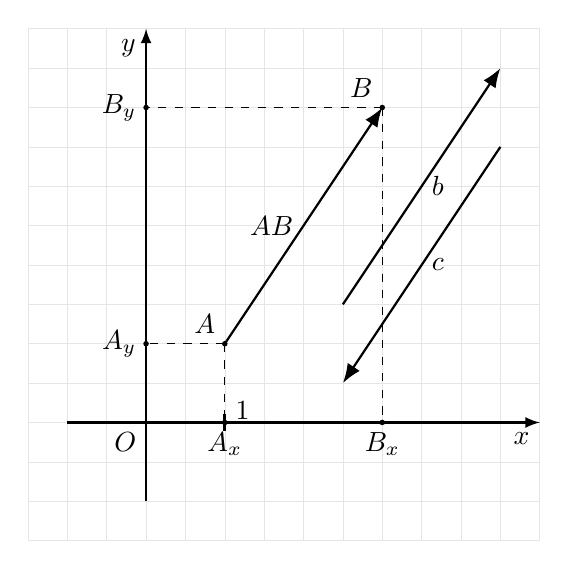
\begin{tikzpicture}[scale=1]
	
	
	\draw[step=.5cm,black!10,very thin] (-1.5,-1.5) grid (5,5);
	
	\draw[-latex, thick] (-1,0) -- (5,0)  node [below left] {$x$};
	\draw[-latex, thick] (0,-1) -- (0,5)  node [below left] {$y$};
	
	\coordinate (O) at (0,0);
	
	\draw (O) node [below left] {$O$};
	
	
	\coordinate (A) at (1,1);
	\coordinate (B) at (3,4);
	\coordinate (Ax) at (A |- O);
	\coordinate (Ay) at (A -| O);
	\coordinate (Bx) at (B |- O);
	\coordinate (By) at (B -| O);
	
	\fill [black] (A) circle [radius=1pt];
	\fill [black] (B) circle [radius=1pt];
	\fill [black] (Ax) circle [radius=1pt];
	\fill [black] (Ay) circle [radius=1pt];
	\fill [black] (Bx) circle [radius=1pt];
	\fill [black] (By) circle [radius=1pt];
	
	\draw[-{Latex[length=7pt]}, thick] (A) -- (B) node [left, midway] {$\vv{AB}$};
	
	\draw (A) node[above left,] {$A$};
	\draw (B) node[above left] {$B$};
	
	\draw (Ax) node [below] {$A_x$};
	\draw (Ay) node [left] {$A_y$};
	\draw (Bx) node [below] {$B_x$};
	\draw (By) node [left] {$B_y$};
	
	
	\draw[dashed] (A) -- (Ax);
	\draw[dashed] (A) -- (Ay);
	\draw[dashed] (B) -- (By);
	\draw[dashed] (B) -- (Bx);
	
	\draw[-{Latex[length=7pt]}, thick] ($(A)+(1.5,0.5)$) -- ($(B)+(1.5,0.5)$) node [right, midway] {$\vv{b}$};
	
	
	\draw[{Latex[length=7pt]}-, thick] ($(A)+(1.5,-0.5)$) -- ($(B)+(1.5,-0.5)$) node [right, midway] {$\vv{c}$};
	
	
	\draw [very thick] (1,0) -- +(up:3pt) -- +(down:3pt) node [above right] {1};
	
	
	
	
	
\end{tikzpicture}
	
\end{document}